% Created by tikzDevice version 0.12.6 on 2025-04-17 10:37:48
% !TEX encoding = UTF-8 Unicode
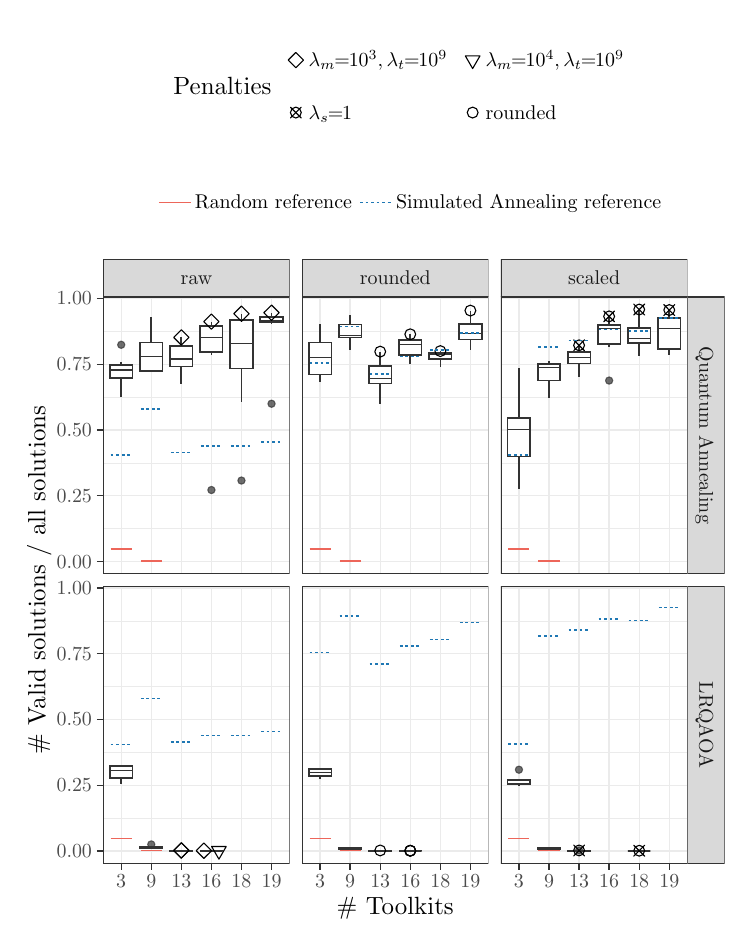
\begin{tikzpicture}[x=1pt,y=1pt]
\definecolor{fillColor}{RGB}{255,255,255}
\path[use as bounding box,fill=fillColor,fill opacity=0.00] (0,0) rectangle (251.81,322.31);
\begin{scope}
\path[clip] (  0.00,  0.00) rectangle (251.81,322.31);
\definecolor{drawColor}{RGB}{255,255,255}
\definecolor{fillColor}{RGB}{255,255,255}

\path[draw=drawColor,line width= 0.5pt,line join=round,line cap=round,fill=fillColor] (  0.00,  0.00) rectangle (251.81,322.31);
\end{scope}
\begin{scope}
\path[clip] ( 27.28,124.93) rectangle ( 94.64,225.00);
\definecolor{fillColor}{RGB}{255,255,255}

\path[fill=fillColor] ( 27.28,124.93) rectangle ( 94.64,225.00);
\definecolor{drawColor}{gray}{0.92}

\path[draw=drawColor,line width= 0.2pt,line join=round] ( 27.28,141.27) --
	( 94.64,141.27);

\path[draw=drawColor,line width= 0.2pt,line join=round] ( 27.28,165.03) --
	( 94.64,165.03);

\path[draw=drawColor,line width= 0.2pt,line join=round] ( 27.28,188.80) --
	( 94.64,188.80);

\path[draw=drawColor,line width= 0.2pt,line join=round] ( 27.28,212.57) --
	( 94.64,212.57);

\path[draw=drawColor,line width= 0.5pt,line join=round] ( 27.28,129.38) --
	( 94.64,129.38);

\path[draw=drawColor,line width= 0.5pt,line join=round] ( 27.28,153.15) --
	( 94.64,153.15);

\path[draw=drawColor,line width= 0.5pt,line join=round] ( 27.28,176.92) --
	( 94.64,176.92);

\path[draw=drawColor,line width= 0.5pt,line join=round] ( 27.28,200.68) --
	( 94.64,200.68);

\path[draw=drawColor,line width= 0.5pt,line join=round] ( 27.28,224.45) --
	( 94.64,224.45);

\path[draw=drawColor,line width= 0.5pt,line join=round] ( 33.80,124.93) --
	( 33.80,225.00);

\path[draw=drawColor,line width= 0.5pt,line join=round] ( 44.66,124.93) --
	( 44.66,225.00);

\path[draw=drawColor,line width= 0.5pt,line join=round] ( 55.52,124.93) --
	( 55.52,225.00);

\path[draw=drawColor,line width= 0.5pt,line join=round] ( 66.39,124.93) --
	( 66.39,225.00);

\path[draw=drawColor,line width= 0.5pt,line join=round] ( 77.25,124.93) --
	( 77.25,225.00);

\path[draw=drawColor,line width= 0.5pt,line join=round] ( 88.12,124.93) --
	( 88.12,225.00);
\definecolor{drawColor}{RGB}{51,51,51}
\definecolor{fillColor}{RGB}{51,51,51}

\path[draw=drawColor,draw opacity=0.70,line width= 0.4pt,line join=round,line cap=round,fill=fillColor,fill opacity=0.70] ( 33.80,207.72) circle (  1.31);
\definecolor{drawColor}{gray}{0.20}

\path[draw=drawColor,line width= 0.6pt,line join=round] ( 33.80,200.44) -- ( 33.80,201.44);

\path[draw=drawColor,line width= 0.6pt,line join=round] ( 33.80,195.74) -- ( 33.80,188.70);
\definecolor{fillColor}{RGB}{255,255,255}

\path[draw=drawColor,line width= 0.6pt,fill=fillColor] ( 29.72,200.44) --
	( 29.72,195.74) --
	( 37.87,195.74) --
	( 37.87,200.44) --
	( 29.72,200.44) --
	cycle;

\path[draw=drawColor,line width= 0.4pt] ( 29.72,198.59) -- ( 37.87,198.59);

\path[draw=drawColor,line width= 0.6pt,line join=round] ( 44.66,208.53) -- ( 44.66,217.60);

\path[draw=drawColor,line width= 0.6pt,line join=round] ( 44.66,198.35) -- ( 44.66,198.21);

\path[draw=drawColor,line width= 0.6pt,fill=fillColor] ( 40.59,208.53) --
	( 40.59,198.35) --
	( 48.73,198.35) --
	( 48.73,208.53) --
	( 40.59,208.53) --
	cycle;

\path[draw=drawColor,line width= 0.4pt] ( 40.59,203.63) -- ( 48.73,203.63);

\path[draw=drawColor,line width= 0.6pt,line join=round] ( 55.52,207.24) -- ( 55.52,210.38);

\path[draw=drawColor,line width= 0.6pt,line join=round] ( 55.52,199.83) -- ( 55.52,193.65);

\path[draw=drawColor,line width= 0.6pt,fill=fillColor] ( 51.45,207.24) --
	( 51.45,199.83) --
	( 59.60,199.83) --
	( 59.60,207.24) --
	( 51.45,207.24) --
	cycle;

\path[draw=drawColor,line width= 0.4pt] ( 51.45,202.58) -- ( 59.60,202.58);
\definecolor{drawColor}{RGB}{51,51,51}
\definecolor{fillColor}{RGB}{51,51,51}

\path[draw=drawColor,draw opacity=0.70,line width= 0.4pt,line join=round,line cap=round,fill=fillColor,fill opacity=0.70] ( 66.39,155.24) circle (  1.31);
\definecolor{drawColor}{gray}{0.20}

\path[draw=drawColor,line width= 0.6pt,line join=round] ( 66.39,214.42) -- ( 66.39,216.08);

\path[draw=drawColor,line width= 0.6pt,line join=round] ( 66.39,205.20) -- ( 66.39,203.91);
\definecolor{fillColor}{RGB}{255,255,255}

\path[draw=drawColor,line width= 0.6pt,fill=fillColor] ( 62.32,214.42) --
	( 62.32,205.20) --
	( 70.46,205.20) --
	( 70.46,214.42) --
	( 62.32,214.42) --
	cycle;

\path[draw=drawColor,line width= 0.4pt] ( 62.32,210.47) -- ( 70.46,210.47);
\definecolor{drawColor}{RGB}{51,51,51}
\definecolor{fillColor}{RGB}{51,51,51}

\path[draw=drawColor,draw opacity=0.70,line width= 0.4pt,line join=round,line cap=round,fill=fillColor,fill opacity=0.70] ( 77.25,158.66) circle (  1.31);
\definecolor{drawColor}{gray}{0.20}

\path[draw=drawColor,line width= 0.6pt,line join=round] ( 77.25,216.56) -- ( 77.25,218.94);

\path[draw=drawColor,line width= 0.6pt,line join=round] ( 77.25,199.16) -- ( 77.25,187.18);
\definecolor{fillColor}{RGB}{255,255,255}

\path[draw=drawColor,line width= 0.6pt,fill=fillColor] ( 73.18,216.56) --
	( 73.18,199.16) --
	( 81.33,199.16) --
	( 81.33,216.56) --
	( 73.18,216.56) --
	cycle;

\path[draw=drawColor,line width= 0.4pt] ( 73.18,208.19) -- ( 81.33,208.19);
\definecolor{drawColor}{RGB}{51,51,51}
\definecolor{fillColor}{RGB}{51,51,51}

\path[draw=drawColor,draw opacity=0.70,line width= 0.4pt,line join=round,line cap=round,fill=fillColor,fill opacity=0.70] ( 88.12,186.42) circle (  1.31);
\definecolor{drawColor}{gray}{0.20}

\path[draw=drawColor,line width= 0.6pt,line join=round] ( 88.12,217.75) -- ( 88.12,219.32);

\path[draw=drawColor,line width= 0.6pt,line join=round] ( 88.12,215.89) -- ( 88.12,215.32);
\definecolor{fillColor}{RGB}{255,255,255}

\path[draw=drawColor,line width= 0.6pt,fill=fillColor] ( 84.04,217.75) --
	( 84.04,215.89) --
	( 92.19,215.89) --
	( 92.19,217.75) --
	( 84.04,217.75) --
	cycle;

\path[draw=drawColor,line width= 0.4pt] ( 84.04,216.56) -- ( 92.19,216.56);
\definecolor{drawColor}{RGB}{0,0,0}

\path[draw=drawColor,line width= 0.4pt,line join=round,line cap=round] ( 74.48,218.94) --
	( 77.25,221.71) --
	( 80.03,218.94) --
	( 77.25,216.16) --
	cycle;

\path[draw=drawColor,line width= 0.4pt,line join=round,line cap=round] ( 63.61,216.08) --
	( 66.39,218.86) --
	( 69.16,216.08) --
	( 66.39,213.31) --
	cycle;

\path[draw=drawColor,line width= 0.4pt,line join=round,line cap=round] ( 85.34,219.32) --
	( 88.12,222.09) --
	( 90.89,219.32) --
	( 88.12,216.54) --
	cycle;

\path[draw=drawColor,line width= 0.4pt,line join=round,line cap=round] ( 52.75,210.38) --
	( 55.52,213.15) --
	( 58.30,210.38) --
	( 55.52,207.60) --
	cycle;
\definecolor{drawColor}{RGB}{237,102,90}

\path[draw=drawColor,line width= 0.6pt,line join=round] ( 29.99,133.95) -- ( 37.60,133.95);

\path[draw=drawColor,line width= 0.6pt,line join=round] ( 40.86,129.57) -- ( 48.46,129.57);
\definecolor{drawColor}{RGB}{31,120,180}

\path[draw=drawColor,line width= 0.6pt,dash pattern=on 1pt off 1pt ,line join=round] ( 40.86,184.44) -- ( 48.46,184.44);

\path[draw=drawColor,line width= 0.6pt,dash pattern=on 1pt off 1pt ,line join=round] ( 73.45,171.06) -- ( 81.06,171.06);

\path[draw=drawColor,line width= 0.6pt,dash pattern=on 1pt off 1pt ,line join=round] ( 51.72,168.78) -- ( 59.33,168.78);

\path[draw=drawColor,line width= 0.6pt,dash pattern=on 1pt off 1pt ,line join=round] ( 62.59,171.17) -- ( 70.19,171.17);

\path[draw=drawColor,line width= 0.6pt,dash pattern=on 1pt off 1pt ,line join=round] ( 29.99,167.92) -- ( 37.60,167.92);

\path[draw=drawColor,line width= 0.6pt,dash pattern=on 1pt off 1pt ,line join=round] ( 84.32,172.54) -- ( 91.92,172.54);
\definecolor{drawColor}{gray}{0.20}

\path[draw=drawColor,line width= 0.5pt,line join=round,line cap=round] ( 27.28,124.93) rectangle ( 94.64,225.00);
\end{scope}
\begin{scope}
\path[clip] ( 27.28, 20.35) rectangle ( 94.64,120.43);
\definecolor{fillColor}{RGB}{255,255,255}

\path[fill=fillColor] ( 27.28, 20.35) rectangle ( 94.64,120.43);
\definecolor{drawColor}{gray}{0.92}

\path[draw=drawColor,line width= 0.2pt,line join=round] ( 27.28, 36.69) --
	( 94.64, 36.69);

\path[draw=drawColor,line width= 0.2pt,line join=round] ( 27.28, 60.46) --
	( 94.64, 60.46);

\path[draw=drawColor,line width= 0.2pt,line join=round] ( 27.28, 84.22) --
	( 94.64, 84.22);

\path[draw=drawColor,line width= 0.2pt,line join=round] ( 27.28,107.99) --
	( 94.64,107.99);

\path[draw=drawColor,line width= 0.5pt,line join=round] ( 27.28, 24.81) --
	( 94.64, 24.81);

\path[draw=drawColor,line width= 0.5pt,line join=round] ( 27.28, 48.57) --
	( 94.64, 48.57);

\path[draw=drawColor,line width= 0.5pt,line join=round] ( 27.28, 72.34) --
	( 94.64, 72.34);

\path[draw=drawColor,line width= 0.5pt,line join=round] ( 27.28, 96.11) --
	( 94.64, 96.11);

\path[draw=drawColor,line width= 0.5pt,line join=round] ( 27.28,119.87) --
	( 94.64,119.87);

\path[draw=drawColor,line width= 0.5pt,line join=round] ( 33.80, 20.35) --
	( 33.80,120.43);

\path[draw=drawColor,line width= 0.5pt,line join=round] ( 44.66, 20.35) --
	( 44.66,120.43);

\path[draw=drawColor,line width= 0.5pt,line join=round] ( 55.52, 20.35) --
	( 55.52,120.43);

\path[draw=drawColor,line width= 0.5pt,line join=round] ( 66.39, 20.35) --
	( 66.39,120.43);

\path[draw=drawColor,line width= 0.5pt,line join=round] ( 77.25, 20.35) --
	( 77.25,120.43);

\path[draw=drawColor,line width= 0.5pt,line join=round] ( 88.12, 20.35) --
	( 88.12,120.43);
\definecolor{drawColor}{gray}{0.20}

\path[draw=drawColor,line width= 0.6pt,line join=round] ( 33.80, 55.56) -- ( 33.80, 55.70);

\path[draw=drawColor,line width= 0.6pt,line join=round] ( 33.80, 51.28) -- ( 33.80, 49.14);

\path[draw=drawColor,line width= 0.6pt,fill=fillColor] ( 29.72, 55.56) --
	( 29.72, 51.28) --
	( 37.87, 51.28) --
	( 37.87, 55.56) --
	( 29.72, 55.56) --
	cycle;

\path[draw=drawColor,line width= 0.4pt] ( 29.72, 53.75) -- ( 37.87, 53.75);
\definecolor{drawColor}{RGB}{51,51,51}
\definecolor{fillColor}{RGB}{51,51,51}

\path[draw=drawColor,draw opacity=0.70,line width= 0.4pt,line join=round,line cap=round,fill=fillColor,fill opacity=0.70] ( 44.66, 27.18) circle (  1.31);
\definecolor{drawColor}{gray}{0.20}

\path[draw=drawColor,line width= 0.6pt,line join=round] ( 44.66, 26.33) -- ( 44.66, 26.33);

\path[draw=drawColor,line width= 0.6pt,line join=round] ( 44.66, 25.95) -- ( 44.66, 25.95);
\definecolor{fillColor}{RGB}{255,255,255}

\path[draw=drawColor,line width= 0.6pt,fill=fillColor] ( 40.59, 26.33) --
	( 40.59, 25.95) --
	( 48.73, 25.95) --
	( 48.73, 26.33) --
	( 40.59, 26.33) --
	cycle;

\path[draw=drawColor,line width= 0.4pt] ( 40.59, 26.14) -- ( 48.73, 26.14);

\path[draw=drawColor,line width= 0.6pt,line join=round] ( 55.52, 25.00) -- ( 55.52, 25.00);

\path[draw=drawColor,line width= 0.6pt,line join=round] ( 55.52, 24.90) -- ( 55.52, 24.90);

\path[draw=drawColor,line width= 0.6pt,fill=fillColor] ( 51.45, 25.00) --
	( 51.45, 24.90) --
	( 59.60, 24.90) --
	( 59.60, 25.00) --
	( 51.45, 25.00) --
	cycle;

\path[draw=drawColor,line width= 0.4pt] ( 51.45, 24.90) -- ( 59.60, 24.90);

\path[draw=drawColor,line width= 0.6pt,line join=round] ( 66.39, 24.90) -- ( 66.39, 24.90);

\path[draw=drawColor,line width= 0.6pt,line join=round] ( 66.39, 24.90) -- ( 66.39, 24.90);

\path[draw=drawColor,line width= 0.6pt,fill=fillColor] ( 62.32, 24.90) --
	( 62.32, 24.90) --
	( 70.46, 24.90) --
	( 70.46, 24.90) --
	( 62.32, 24.90) --
	cycle;

\path[draw=drawColor,line width= 0.4pt] ( 62.32, 24.90) -- ( 70.46, 24.90);
\definecolor{drawColor}{RGB}{0,0,0}

\path[draw=drawColor,line width= 0.4pt,line join=round,line cap=round] ( 60.90, 24.90) --
	( 63.67, 27.68) --
	( 66.45, 24.90) --
	( 63.67, 22.13) --
	cycle;

\path[draw=drawColor,line width= 0.4pt,line join=round,line cap=round] ( 52.75, 25.00) --
	( 55.52, 27.77) --
	( 58.30, 25.00) --
	( 55.52, 22.22) --
	cycle;

\path[draw=drawColor,line width= 0.4pt,line join=round,line cap=round] ( 69.11, 21.85) --
	( 71.75, 26.43) --
	( 66.46, 26.43) --
	cycle;

\path[draw=drawColor,line width= 0.4pt,line join=round,line cap=round] ( 52.75, 25.00) --
	( 55.52, 27.77) --
	( 58.30, 25.00) --
	( 55.52, 22.22) --
	cycle;
\definecolor{drawColor}{RGB}{237,102,90}

\path[draw=drawColor,line width= 0.6pt,line join=round] ( 29.99, 29.37) -- ( 37.60, 29.37);

\path[draw=drawColor,line width= 0.6pt,line join=round] ( 40.86, 25.00) -- ( 48.46, 25.00);
\definecolor{drawColor}{RGB}{31,120,180}

\path[draw=drawColor,line width= 0.6pt,dash pattern=on 1pt off 1pt ,line join=round] ( 40.86, 79.86) -- ( 48.46, 79.86);

\path[draw=drawColor,line width= 0.6pt,dash pattern=on 1pt off 1pt ,line join=round] ( 73.45, 66.49) -- ( 81.06, 66.49);

\path[draw=drawColor,line width= 0.6pt,dash pattern=on 1pt off 1pt ,line join=round] ( 51.72, 64.21) -- ( 59.33, 64.21);

\path[draw=drawColor,line width= 0.6pt,dash pattern=on 1pt off 1pt ,line join=round] ( 62.59, 66.59) -- ( 70.19, 66.59);

\path[draw=drawColor,line width= 0.6pt,dash pattern=on 1pt off 1pt ,line join=round] ( 29.99, 63.34) -- ( 37.60, 63.34);

\path[draw=drawColor,line width= 0.6pt,dash pattern=on 1pt off 1pt ,line join=round] ( 84.32, 67.97) -- ( 91.92, 67.97);
\definecolor{drawColor}{gray}{0.20}

\path[draw=drawColor,line width= 0.5pt,line join=round,line cap=round] ( 27.28, 20.35) rectangle ( 94.64,120.43);
\end{scope}
\begin{scope}
\path[clip] ( 99.14,124.93) rectangle (166.50,225.00);
\definecolor{fillColor}{RGB}{255,255,255}

\path[fill=fillColor] ( 99.14,124.93) rectangle (166.50,225.00);
\definecolor{drawColor}{gray}{0.92}

\path[draw=drawColor,line width= 0.2pt,line join=round] ( 99.14,141.27) --
	(166.50,141.27);

\path[draw=drawColor,line width= 0.2pt,line join=round] ( 99.14,165.03) --
	(166.50,165.03);

\path[draw=drawColor,line width= 0.2pt,line join=round] ( 99.14,188.80) --
	(166.50,188.80);

\path[draw=drawColor,line width= 0.2pt,line join=round] ( 99.14,212.57) --
	(166.50,212.57);

\path[draw=drawColor,line width= 0.5pt,line join=round] ( 99.14,129.38) --
	(166.50,129.38);

\path[draw=drawColor,line width= 0.5pt,line join=round] ( 99.14,153.15) --
	(166.50,153.15);

\path[draw=drawColor,line width= 0.5pt,line join=round] ( 99.14,176.92) --
	(166.50,176.92);

\path[draw=drawColor,line width= 0.5pt,line join=round] ( 99.14,200.68) --
	(166.50,200.68);

\path[draw=drawColor,line width= 0.5pt,line join=round] ( 99.14,224.45) --
	(166.50,224.45);

\path[draw=drawColor,line width= 0.5pt,line join=round] (105.66,124.93) --
	(105.66,225.00);

\path[draw=drawColor,line width= 0.5pt,line join=round] (116.52,124.93) --
	(116.52,225.00);

\path[draw=drawColor,line width= 0.5pt,line join=round] (127.39,124.93) --
	(127.39,225.00);

\path[draw=drawColor,line width= 0.5pt,line join=round] (138.25,124.93) --
	(138.25,225.00);

\path[draw=drawColor,line width= 0.5pt,line join=round] (149.12,124.93) --
	(149.12,225.00);

\path[draw=drawColor,line width= 0.5pt,line join=round] (159.98,124.93) --
	(159.98,225.00);
\definecolor{drawColor}{gray}{0.20}

\path[draw=drawColor,line width= 0.6pt,line join=round] (105.66,208.53) -- (105.66,215.32);

\path[draw=drawColor,line width= 0.6pt,line join=round] (105.66,196.93) -- (105.66,194.41);

\path[draw=drawColor,line width= 0.6pt,fill=fillColor] (101.58,208.53) --
	(101.58,196.93) --
	(109.73,196.93) --
	(109.73,208.53) --
	(101.58,208.53) --
	cycle;

\path[draw=drawColor,line width= 0.4pt] (101.58,203.25) -- (109.73,203.25);

\path[draw=drawColor,line width= 0.6pt,line join=round] (116.52,215.08) -- (116.52,218.36);

\path[draw=drawColor,line width= 0.6pt,line join=round] (116.52,210.33) -- (116.52,205.82);

\path[draw=drawColor,line width= 0.6pt,fill=fillColor] (112.45,215.08) --
	(112.45,210.33) --
	(120.60,210.33) --
	(120.60,215.08) --
	(112.45,215.08) --
	cycle;

\path[draw=drawColor,line width= 0.4pt] (112.45,210.95) -- (120.60,210.95);

\path[draw=drawColor,line width= 0.6pt,line join=round] (127.39,200.16) -- (127.39,205.25);

\path[draw=drawColor,line width= 0.6pt,line join=round] (127.39,193.70) -- (127.39,186.23);

\path[draw=drawColor,line width= 0.6pt,fill=fillColor] (123.31,200.16) --
	(123.31,193.70) --
	(131.46,193.70) --
	(131.46,200.16) --
	(123.31,200.16) --
	cycle;

\path[draw=drawColor,line width= 0.4pt] (123.31,195.64) -- (131.46,195.64);

\path[draw=drawColor,line width= 0.6pt,line join=round] (138.25,209.52) -- (138.25,211.52);

\path[draw=drawColor,line width= 0.6pt,line join=round] (138.25,204.10) -- (138.25,200.68);

\path[draw=drawColor,line width= 0.6pt,fill=fillColor] (134.18,209.52) --
	(134.18,204.10) --
	(142.33,204.10) --
	(142.33,209.52) --
	(134.18,209.52) --
	cycle;

\path[draw=drawColor,line width= 0.4pt] (134.18,207.81) -- (142.33,207.81);

\path[draw=drawColor,line width= 0.6pt,line join=round] (149.12,204.68) -- (149.12,205.44);

\path[draw=drawColor,line width= 0.6pt,line join=round] (149.12,202.49) -- (149.12,199.54);

\path[draw=drawColor,line width= 0.6pt,fill=fillColor] (145.04,204.68) --
	(145.04,202.49) --
	(153.19,202.49) --
	(153.19,204.68) --
	(145.04,204.68) --
	cycle;

\path[draw=drawColor,line width= 0.4pt] (145.04,204.29) -- (153.19,204.29);

\path[draw=drawColor,line width= 0.6pt,line join=round] (159.98,215.32) -- (159.98,220.08);

\path[draw=drawColor,line width= 0.6pt,line join=round] (159.98,209.57) -- (159.98,206.01);

\path[draw=drawColor,line width= 0.6pt,fill=fillColor] (155.91,215.32) --
	(155.91,209.57) --
	(164.05,209.57) --
	(164.05,215.32) --
	(155.91,215.32) --
	cycle;

\path[draw=drawColor,line width= 0.4pt] (155.91,211.71) -- (164.05,211.71);
\definecolor{drawColor}{RGB}{0,0,0}

\path[draw=drawColor,line width= 0.4pt,line join=round,line cap=round] (138.25,211.52) circle (  1.96);

\path[draw=drawColor,line width= 0.4pt,line join=round,line cap=round] (149.12,205.44) circle (  1.96);

\path[draw=drawColor,line width= 0.4pt,line join=round,line cap=round] (127.39,205.25) circle (  1.96);

\path[draw=drawColor,line width= 0.4pt,line join=round,line cap=round] (159.98,220.08) circle (  1.96);
\definecolor{drawColor}{RGB}{237,102,90}

\path[draw=drawColor,line width= 0.6pt,line join=round] (112.72,129.57) -- (120.32,129.57);

\path[draw=drawColor,line width= 0.6pt,line join=round] (101.85,133.95) -- (109.46,133.95);
\definecolor{drawColor}{RGB}{31,120,180}

\path[draw=drawColor,line width= 0.6pt,dash pattern=on 1pt off 1pt ,line join=round] (112.72,214.37) -- (120.32,214.37);

\path[draw=drawColor,line width= 0.6pt,dash pattern=on 1pt off 1pt ,line join=round] (134.45,203.53) -- (142.05,203.53);

\path[draw=drawColor,line width= 0.6pt,dash pattern=on 1pt off 1pt ,line join=round] (156.18,211.90) -- (163.78,211.90);

\path[draw=drawColor,line width= 0.6pt,dash pattern=on 1pt off 1pt ,line join=round] (101.85,201.06) -- (109.46,201.06);

\path[draw=drawColor,line width= 0.6pt,dash pattern=on 1pt off 1pt ,line join=round] (145.31,205.82) -- (152.92,205.82);

\path[draw=drawColor,line width= 0.6pt,dash pattern=on 1pt off 1pt ,line join=round] (123.58,197.07) -- (131.19,197.07);
\definecolor{drawColor}{gray}{0.20}

\path[draw=drawColor,line width= 0.5pt,line join=round,line cap=round] ( 99.14,124.93) rectangle (166.50,225.00);
\end{scope}
\begin{scope}
\path[clip] ( 99.14, 20.35) rectangle (166.50,120.43);
\definecolor{fillColor}{RGB}{255,255,255}

\path[fill=fillColor] ( 99.14, 20.35) rectangle (166.50,120.43);
\definecolor{drawColor}{gray}{0.92}

\path[draw=drawColor,line width= 0.2pt,line join=round] ( 99.14, 36.69) --
	(166.50, 36.69);

\path[draw=drawColor,line width= 0.2pt,line join=round] ( 99.14, 60.46) --
	(166.50, 60.46);

\path[draw=drawColor,line width= 0.2pt,line join=round] ( 99.14, 84.22) --
	(166.50, 84.22);

\path[draw=drawColor,line width= 0.2pt,line join=round] ( 99.14,107.99) --
	(166.50,107.99);

\path[draw=drawColor,line width= 0.5pt,line join=round] ( 99.14, 24.81) --
	(166.50, 24.81);

\path[draw=drawColor,line width= 0.5pt,line join=round] ( 99.14, 48.57) --
	(166.50, 48.57);

\path[draw=drawColor,line width= 0.5pt,line join=round] ( 99.14, 72.34) --
	(166.50, 72.34);

\path[draw=drawColor,line width= 0.5pt,line join=round] ( 99.14, 96.11) --
	(166.50, 96.11);

\path[draw=drawColor,line width= 0.5pt,line join=round] ( 99.14,119.87) --
	(166.50,119.87);

\path[draw=drawColor,line width= 0.5pt,line join=round] (105.66, 20.35) --
	(105.66,120.43);

\path[draw=drawColor,line width= 0.5pt,line join=round] (116.52, 20.35) --
	(116.52,120.43);

\path[draw=drawColor,line width= 0.5pt,line join=round] (127.39, 20.35) --
	(127.39,120.43);

\path[draw=drawColor,line width= 0.5pt,line join=round] (138.25, 20.35) --
	(138.25,120.43);

\path[draw=drawColor,line width= 0.5pt,line join=round] (149.12, 20.35) --
	(149.12,120.43);

\path[draw=drawColor,line width= 0.5pt,line join=round] (159.98, 20.35) --
	(159.98,120.43);
\definecolor{drawColor}{gray}{0.20}

\path[draw=drawColor,line width= 0.6pt,line join=round] (105.66, 54.37) -- (105.66, 54.37);

\path[draw=drawColor,line width= 0.6pt,line join=round] (105.66, 51.88) -- (105.66, 50.95);

\path[draw=drawColor,line width= 0.6pt,fill=fillColor] (101.58, 54.37) --
	(101.58, 51.88) --
	(109.73, 51.88) --
	(109.73, 54.37) --
	(101.58, 54.37) --
	cycle;

\path[draw=drawColor,line width= 0.4pt] (101.58, 53.28) -- (109.73, 53.28);

\path[draw=drawColor,line width= 0.6pt,line join=round] (116.52, 25.92) -- (116.52, 26.14);

\path[draw=drawColor,line width= 0.6pt,line join=round] (116.52, 25.64) -- (116.52, 25.57);

\path[draw=drawColor,line width= 0.6pt,fill=fillColor] (112.45, 25.92) --
	(112.45, 25.64) --
	(120.60, 25.64) --
	(120.60, 25.92) --
	(112.45, 25.92) --
	cycle;

\path[draw=drawColor,line width= 0.4pt] (112.45, 25.76) -- (120.60, 25.76);

\path[draw=drawColor,line width= 0.6pt,line join=round] (127.39, 24.95) -- (127.39, 25.00);

\path[draw=drawColor,line width= 0.6pt,line join=round] (127.39, 24.90) -- (127.39, 24.90);

\path[draw=drawColor,line width= 0.6pt,fill=fillColor] (123.31, 24.95) --
	(123.31, 24.90) --
	(131.46, 24.90) --
	(131.46, 24.95) --
	(123.31, 24.95) --
	cycle;

\path[draw=drawColor,line width= 0.4pt] (123.31, 24.90) -- (131.46, 24.90);

\path[draw=drawColor,line width= 0.6pt,line join=round] (138.25, 24.90) -- (138.25, 24.90);

\path[draw=drawColor,line width= 0.6pt,line join=round] (138.25, 24.90) -- (138.25, 24.90);

\path[draw=drawColor,line width= 0.6pt,fill=fillColor] (134.18, 24.90) --
	(134.18, 24.90) --
	(142.33, 24.90) --
	(142.33, 24.90) --
	(134.18, 24.90) --
	cycle;

\path[draw=drawColor,line width= 0.4pt] (134.18, 24.90) -- (142.33, 24.90);
\definecolor{drawColor}{RGB}{0,0,0}

\path[draw=drawColor,line width= 0.4pt,line join=round,line cap=round] (138.25, 24.90) circle (  1.96);

\path[draw=drawColor,line width= 0.4pt,line join=round,line cap=round] (138.25, 24.90) circle (  1.96);

\path[draw=drawColor,line width= 0.4pt,line join=round,line cap=round] (127.39, 25.00) circle (  1.96);

\path[draw=drawColor,line width= 0.4pt,line join=round,line cap=round] (138.25, 24.90) circle (  1.96);
\definecolor{drawColor}{RGB}{237,102,90}

\path[draw=drawColor,line width= 0.6pt,line join=round] (112.72, 25.00) -- (120.32, 25.00);

\path[draw=drawColor,line width= 0.6pt,line join=round] (101.85, 29.37) -- (109.46, 29.37);
\definecolor{drawColor}{RGB}{31,120,180}

\path[draw=drawColor,line width= 0.6pt,dash pattern=on 1pt off 1pt ,line join=round] (112.72,109.80) -- (120.32,109.80);

\path[draw=drawColor,line width= 0.6pt,dash pattern=on 1pt off 1pt ,line join=round] (134.45, 98.96) -- (142.05, 98.96);

\path[draw=drawColor,line width= 0.6pt,dash pattern=on 1pt off 1pt ,line join=round] (156.18,107.32) -- (163.78,107.32);

\path[draw=drawColor,line width= 0.6pt,dash pattern=on 1pt off 1pt ,line join=round] (101.85, 96.49) -- (109.46, 96.49);

\path[draw=drawColor,line width= 0.6pt,dash pattern=on 1pt off 1pt ,line join=round] (145.31,101.24) -- (152.92,101.24);

\path[draw=drawColor,line width= 0.6pt,dash pattern=on 1pt off 1pt ,line join=round] (123.58, 92.49) -- (131.19, 92.49);
\definecolor{drawColor}{gray}{0.20}

\path[draw=drawColor,line width= 0.5pt,line join=round,line cap=round] ( 99.14, 20.35) rectangle (166.50,120.43);
\end{scope}
\begin{scope}
\path[clip] (171.00,124.93) rectangle (238.36,225.00);
\definecolor{fillColor}{RGB}{255,255,255}

\path[fill=fillColor] (171.00,124.93) rectangle (238.36,225.00);
\definecolor{drawColor}{gray}{0.92}

\path[draw=drawColor,line width= 0.2pt,line join=round] (171.00,141.27) --
	(238.36,141.27);

\path[draw=drawColor,line width= 0.2pt,line join=round] (171.00,165.03) --
	(238.36,165.03);

\path[draw=drawColor,line width= 0.2pt,line join=round] (171.00,188.80) --
	(238.36,188.80);

\path[draw=drawColor,line width= 0.2pt,line join=round] (171.00,212.57) --
	(238.36,212.57);

\path[draw=drawColor,line width= 0.5pt,line join=round] (171.00,129.38) --
	(238.36,129.38);

\path[draw=drawColor,line width= 0.5pt,line join=round] (171.00,153.15) --
	(238.36,153.15);

\path[draw=drawColor,line width= 0.5pt,line join=round] (171.00,176.92) --
	(238.36,176.92);

\path[draw=drawColor,line width= 0.5pt,line join=round] (171.00,200.68) --
	(238.36,200.68);

\path[draw=drawColor,line width= 0.5pt,line join=round] (171.00,224.45) --
	(238.36,224.45);

\path[draw=drawColor,line width= 0.5pt,line join=round] (177.52,124.93) --
	(177.52,225.00);

\path[draw=drawColor,line width= 0.5pt,line join=round] (188.38,124.93) --
	(188.38,225.00);

\path[draw=drawColor,line width= 0.5pt,line join=round] (199.25,124.93) --
	(199.25,225.00);

\path[draw=drawColor,line width= 0.5pt,line join=round] (210.11,124.93) --
	(210.11,225.00);

\path[draw=drawColor,line width= 0.5pt,line join=round] (220.98,124.93) --
	(220.98,225.00);

\path[draw=drawColor,line width= 0.5pt,line join=round] (231.84,124.93) --
	(231.84,225.00);
\definecolor{drawColor}{gray}{0.20}

\path[draw=drawColor,line width= 0.6pt,line join=round] (177.52,181.19) -- (177.52,199.35);

\path[draw=drawColor,line width= 0.6pt,line join=round] (177.52,167.31) -- (177.52,155.43);

\path[draw=drawColor,line width= 0.6pt,fill=fillColor] (173.44,181.19) --
	(173.44,167.31) --
	(181.59,167.31) --
	(181.59,181.19) --
	(173.44,181.19) --
	cycle;

\path[draw=drawColor,line width= 0.4pt] (173.44,177.11) -- (181.59,177.11);

\path[draw=drawColor,line width= 0.6pt,line join=round] (188.38,200.87) -- (188.38,201.82);

\path[draw=drawColor,line width= 0.6pt,line join=round] (188.38,194.84) -- (188.38,188.32);

\path[draw=drawColor,line width= 0.6pt,fill=fillColor] (184.31,200.87) --
	(184.31,194.84) --
	(192.46,194.84) --
	(192.46,200.87) --
	(184.31,200.87) --
	cycle;

\path[draw=drawColor,line width= 0.4pt] (184.31,199.35) -- (192.46,199.35);

\path[draw=drawColor,line width= 0.6pt,line join=round] (199.25,205.10) -- (199.25,207.53);

\path[draw=drawColor,line width= 0.6pt,line join=round] (199.25,200.92) -- (199.25,196.12);

\path[draw=drawColor,line width= 0.6pt,fill=fillColor] (195.17,205.10) --
	(195.17,200.92) --
	(203.32,200.92) --
	(203.32,205.10) --
	(195.17,205.10) --
	cycle;

\path[draw=drawColor,line width= 0.4pt] (195.17,203.15) -- (203.32,203.15);
\definecolor{drawColor}{RGB}{51,51,51}
\definecolor{fillColor}{RGB}{51,51,51}

\path[draw=drawColor,draw opacity=0.70,line width= 0.4pt,line join=round,line cap=round,fill=fillColor,fill opacity=0.70] (210.11,194.79) circle (  1.31);
\definecolor{drawColor}{gray}{0.20}

\path[draw=drawColor,line width= 0.6pt,line join=round] (210.11,214.80) -- (210.11,217.98);

\path[draw=drawColor,line width= 0.6pt,line join=round] (210.11,207.95) -- (210.11,206.96);
\definecolor{fillColor}{RGB}{255,255,255}

\path[draw=drawColor,line width= 0.6pt,fill=fillColor] (206.04,214.80) --
	(206.04,207.95) --
	(214.19,207.95) --
	(214.19,214.80) --
	(206.04,214.80) --
	cycle;

\path[draw=drawColor,line width= 0.4pt] (206.04,213.52) -- (214.19,213.52);

\path[draw=drawColor,line width= 0.6pt,line join=round] (220.98,213.71) -- (220.98,220.46);

\path[draw=drawColor,line width= 0.6pt,line join=round] (220.98,208.29) -- (220.98,203.72);

\path[draw=drawColor,line width= 0.6pt,fill=fillColor] (216.90,213.71) --
	(216.90,208.29) --
	(225.05,208.29) --
	(225.05,213.71) --
	(216.90,213.71) --
	cycle;

\path[draw=drawColor,line width= 0.4pt] (216.90,210.09) -- (225.05,210.09);

\path[draw=drawColor,line width= 0.6pt,line join=round] (231.84,217.41) -- (231.84,220.27);

\path[draw=drawColor,line width= 0.6pt,line join=round] (231.84,206.24) -- (231.84,203.91);

\path[draw=drawColor,line width= 0.6pt,fill=fillColor] (227.77,217.41) --
	(227.77,206.24) --
	(235.92,206.24) --
	(235.92,217.41) --
	(227.77,217.41) --
	cycle;

\path[draw=drawColor,line width= 0.4pt] (227.77,213.71) -- (235.92,213.71);
\definecolor{drawColor}{RGB}{0,0,0}

\path[draw=drawColor,line width= 0.4pt,line join=round,line cap=round] (220.98,220.46) circle (  1.96);

\path[draw=drawColor,line width= 0.4pt,line join=round,line cap=round] (219.02,218.49) -- (222.94,222.42);

\path[draw=drawColor,line width= 0.4pt,line join=round,line cap=round] (219.02,222.42) -- (222.94,218.49);

\path[draw=drawColor,line width= 0.4pt,line join=round,line cap=round] (199.25,207.53) circle (  1.96);

\path[draw=drawColor,line width= 0.4pt,line join=round,line cap=round] (197.29,205.56) -- (201.21,209.49);

\path[draw=drawColor,line width= 0.4pt,line join=round,line cap=round] (197.29,209.49) -- (201.21,205.56);

\path[draw=drawColor,line width= 0.4pt,line join=round,line cap=round] (210.11,217.98) circle (  1.96);

\path[draw=drawColor,line width= 0.4pt,line join=round,line cap=round] (208.15,216.02) -- (212.07,219.95);

\path[draw=drawColor,line width= 0.4pt,line join=round,line cap=round] (208.15,219.95) -- (212.07,216.02);

\path[draw=drawColor,line width= 0.4pt,line join=round,line cap=round] (231.84,220.27) circle (  1.96);

\path[draw=drawColor,line width= 0.4pt,line join=round,line cap=round] (229.88,218.30) -- (233.80,222.23);

\path[draw=drawColor,line width= 0.4pt,line join=round,line cap=round] (229.88,222.23) -- (233.80,218.30);
\definecolor{drawColor}{RGB}{237,102,90}

\path[draw=drawColor,line width= 0.6pt,line join=round] (184.58,129.57) -- (192.19,129.57);

\path[draw=drawColor,line width= 0.6pt,line join=round] (173.72,133.95) -- (181.32,133.95);
\definecolor{drawColor}{RGB}{31,120,180}

\path[draw=drawColor,line width= 0.6pt,dash pattern=on 1pt off 1pt ,line join=round] (217.17,212.66) -- (224.78,212.66);

\path[draw=drawColor,line width= 0.6pt,dash pattern=on 1pt off 1pt ,line join=round] (195.45,209.24) -- (203.05,209.24);

\path[draw=drawColor,line width= 0.6pt,dash pattern=on 1pt off 1pt ,line join=round] (184.58,206.96) -- (192.19,206.96);

\path[draw=drawColor,line width= 0.6pt,dash pattern=on 1pt off 1pt ,line join=round] (206.31,213.23) -- (213.92,213.23);

\path[draw=drawColor,line width= 0.6pt,dash pattern=on 1pt off 1pt ,line join=round] (228.04,217.41) -- (235.64,217.41);

\path[draw=drawColor,line width= 0.6pt,dash pattern=on 1pt off 1pt ,line join=round] (173.72,167.98) -- (181.32,167.98);
\definecolor{drawColor}{gray}{0.20}

\path[draw=drawColor,line width= 0.5pt,line join=round,line cap=round] (171.00,124.93) rectangle (238.36,225.00);
\end{scope}
\begin{scope}
\path[clip] (171.00, 20.35) rectangle (238.36,120.43);
\definecolor{fillColor}{RGB}{255,255,255}

\path[fill=fillColor] (171.00, 20.35) rectangle (238.36,120.43);
\definecolor{drawColor}{gray}{0.92}

\path[draw=drawColor,line width= 0.2pt,line join=round] (171.00, 36.69) --
	(238.36, 36.69);

\path[draw=drawColor,line width= 0.2pt,line join=round] (171.00, 60.46) --
	(238.36, 60.46);

\path[draw=drawColor,line width= 0.2pt,line join=round] (171.00, 84.22) --
	(238.36, 84.22);

\path[draw=drawColor,line width= 0.2pt,line join=round] (171.00,107.99) --
	(238.36,107.99);

\path[draw=drawColor,line width= 0.5pt,line join=round] (171.00, 24.81) --
	(238.36, 24.81);

\path[draw=drawColor,line width= 0.5pt,line join=round] (171.00, 48.57) --
	(238.36, 48.57);

\path[draw=drawColor,line width= 0.5pt,line join=round] (171.00, 72.34) --
	(238.36, 72.34);

\path[draw=drawColor,line width= 0.5pt,line join=round] (171.00, 96.11) --
	(238.36, 96.11);

\path[draw=drawColor,line width= 0.5pt,line join=round] (171.00,119.87) --
	(238.36,119.87);

\path[draw=drawColor,line width= 0.5pt,line join=round] (177.52, 20.35) --
	(177.52,120.43);

\path[draw=drawColor,line width= 0.5pt,line join=round] (188.38, 20.35) --
	(188.38,120.43);

\path[draw=drawColor,line width= 0.5pt,line join=round] (199.25, 20.35) --
	(199.25,120.43);

\path[draw=drawColor,line width= 0.5pt,line join=round] (210.11, 20.35) --
	(210.11,120.43);

\path[draw=drawColor,line width= 0.5pt,line join=round] (220.98, 20.35) --
	(220.98,120.43);

\path[draw=drawColor,line width= 0.5pt,line join=round] (231.84, 20.35) --
	(231.84,120.43);
\definecolor{drawColor}{RGB}{51,51,51}
\definecolor{fillColor}{RGB}{51,51,51}

\path[draw=drawColor,draw opacity=0.70,line width= 0.4pt,line join=round,line cap=round,fill=fillColor,fill opacity=0.70] (177.52, 54.18) circle (  1.31);
\definecolor{drawColor}{gray}{0.20}

\path[draw=drawColor,line width= 0.6pt,line join=round] (177.52, 50.49) -- (177.52, 50.49);

\path[draw=drawColor,line width= 0.6pt,line join=round] (177.52, 48.77) -- (177.52, 48.22);
\definecolor{fillColor}{RGB}{255,255,255}

\path[draw=drawColor,line width= 0.6pt,fill=fillColor] (173.44, 50.49) --
	(173.44, 48.77) --
	(181.59, 48.77) --
	(181.59, 50.49) --
	(173.44, 50.49) --
	cycle;

\path[draw=drawColor,line width= 0.4pt] (173.44, 49.11) -- (181.59, 49.11);

\path[draw=drawColor,line width= 0.6pt,line join=round] (188.38, 25.95) -- (188.38, 26.23);

\path[draw=drawColor,line width= 0.6pt,line join=round] (188.38, 25.64) -- (188.38, 25.57);

\path[draw=drawColor,line width= 0.6pt,fill=fillColor] (184.31, 25.95) --
	(184.31, 25.64) --
	(192.46, 25.64) --
	(192.46, 25.95) --
	(184.31, 25.95) --
	cycle;

\path[draw=drawColor,line width= 0.4pt] (184.31, 25.76) -- (192.46, 25.76);
\definecolor{drawColor}{RGB}{51,51,51}
\definecolor{fillColor}{RGB}{51,51,51}

\path[draw=drawColor,draw opacity=0.70,line width= 0.4pt,line join=round,line cap=round,fill=fillColor,fill opacity=0.70] (199.25, 25.00) circle (  1.31);
\definecolor{drawColor}{gray}{0.20}

\path[draw=drawColor,line width= 0.6pt,line join=round] (199.25, 24.93) -- (199.25, 24.93);

\path[draw=drawColor,line width= 0.6pt,line join=round] (199.25, 24.90) -- (199.25, 24.90);
\definecolor{fillColor}{RGB}{255,255,255}

\path[draw=drawColor,line width= 0.6pt,fill=fillColor] (195.17, 24.93) --
	(195.17, 24.90) --
	(203.32, 24.90) --
	(203.32, 24.93) --
	(195.17, 24.93) --
	cycle;

\path[draw=drawColor,line width= 0.4pt] (195.17, 24.90) -- (203.32, 24.90);

\path[draw=drawColor,line width= 0.6pt,line join=round] (220.98, 24.90) -- (220.98, 24.90);

\path[draw=drawColor,line width= 0.6pt,line join=round] (220.98, 24.90) -- (220.98, 24.90);

\path[draw=drawColor,line width= 0.6pt,fill=fillColor] (216.90, 24.90) --
	(216.90, 24.90) --
	(225.05, 24.90) --
	(225.05, 24.90) --
	(216.90, 24.90) --
	cycle;

\path[draw=drawColor,line width= 0.4pt] (216.90, 24.90) -- (225.05, 24.90);
\definecolor{drawColor}{RGB}{0,0,0}

\path[draw=drawColor,line width= 0.4pt,line join=round,line cap=round] (220.98, 24.90) circle (  1.96);

\path[draw=drawColor,line width= 0.4pt,line join=round,line cap=round] (219.02, 22.94) -- (222.94, 26.86);

\path[draw=drawColor,line width= 0.4pt,line join=round,line cap=round] (219.02, 26.86) -- (222.94, 22.94);

\path[draw=drawColor,line width= 0.4pt,line join=round,line cap=round] (199.25, 25.00) circle (  1.96);

\path[draw=drawColor,line width= 0.4pt,line join=round,line cap=round] (197.29, 23.03) -- (201.21, 26.96);

\path[draw=drawColor,line width= 0.4pt,line join=round,line cap=round] (197.29, 26.96) -- (201.21, 23.03);
\definecolor{drawColor}{RGB}{237,102,90}

\path[draw=drawColor,line width= 0.6pt,line join=round] (184.58, 25.00) -- (192.19, 25.00);

\path[draw=drawColor,line width= 0.6pt,line join=round] (173.72, 29.37) -- (181.32, 29.37);
\definecolor{drawColor}{RGB}{31,120,180}

\path[draw=drawColor,line width= 0.6pt,dash pattern=on 1pt off 1pt ,line join=round] (217.17,108.08) -- (224.78,108.08);

\path[draw=drawColor,line width= 0.6pt,dash pattern=on 1pt off 1pt ,line join=round] (195.45,104.66) -- (203.05,104.66);

\path[draw=drawColor,line width= 0.6pt,dash pattern=on 1pt off 1pt ,line join=round] (184.58,102.38) -- (192.19,102.38);

\path[draw=drawColor,line width= 0.6pt,dash pattern=on 1pt off 1pt ,line join=round] (206.31,108.66) -- (213.92,108.66);

\path[draw=drawColor,line width= 0.6pt,dash pattern=on 1pt off 1pt ,line join=round] (228.04,112.84) -- (235.64,112.84);

\path[draw=drawColor,line width= 0.6pt,dash pattern=on 1pt off 1pt ,line join=round] (173.72, 63.40) -- (181.32, 63.40);
\definecolor{drawColor}{gray}{0.20}

\path[draw=drawColor,line width= 0.5pt,line join=round,line cap=round] (171.00, 20.35) rectangle (238.36,120.43);
\end{scope}
\begin{scope}
\path[clip] ( 27.28,225.00) rectangle ( 94.64,238.45);
\definecolor{drawColor}{gray}{0.20}
\definecolor{fillColor}{gray}{0.85}

\path[draw=drawColor,line width= 0.5pt,line join=round,line cap=round,fill=fillColor] ( 27.28,225.00) rectangle ( 94.64,238.45);
\definecolor{drawColor}{gray}{0.10}

\node[text=drawColor,anchor=base,inner sep=0pt, outer sep=0pt, scale=  0.72] at ( 60.96,229.38) {raw};
\end{scope}
\begin{scope}
\path[clip] ( 99.14,225.00) rectangle (166.50,238.45);
\definecolor{drawColor}{gray}{0.20}
\definecolor{fillColor}{gray}{0.85}

\path[draw=drawColor,line width= 0.5pt,line join=round,line cap=round,fill=fillColor] ( 99.14,225.00) rectangle (166.50,238.45);
\definecolor{drawColor}{gray}{0.10}

\node[text=drawColor,anchor=base,inner sep=0pt, outer sep=0pt, scale=  0.72] at (132.82,229.38) {rounded};
\end{scope}
\begin{scope}
\path[clip] (171.00,225.00) rectangle (238.36,238.45);
\definecolor{drawColor}{gray}{0.20}
\definecolor{fillColor}{gray}{0.85}

\path[draw=drawColor,line width= 0.5pt,line join=round,line cap=round,fill=fillColor] (171.00,225.00) rectangle (238.36,238.45);
\definecolor{drawColor}{gray}{0.10}

\node[text=drawColor,anchor=base,inner sep=0pt, outer sep=0pt, scale=  0.72] at (204.68,229.38) {scaled};
\end{scope}
\begin{scope}
\path[clip] (238.36,124.93) rectangle (251.81,225.00);
\definecolor{drawColor}{gray}{0.20}
\definecolor{fillColor}{gray}{0.85}

\path[draw=drawColor,line width= 0.5pt,line join=round,line cap=round,fill=fillColor] (238.36,124.93) rectangle (251.81,225.00);
\definecolor{drawColor}{gray}{0.10}

\node[text=drawColor,rotate=-90.00,anchor=base,inner sep=0pt, outer sep=0pt, scale=  0.72] at (242.74,174.97) {Quantum Annealing};
\end{scope}
\begin{scope}
\path[clip] (238.36, 20.35) rectangle (251.81,120.43);
\definecolor{drawColor}{gray}{0.20}
\definecolor{fillColor}{gray}{0.85}

\path[draw=drawColor,line width= 0.5pt,line join=round,line cap=round,fill=fillColor] (238.36, 20.35) rectangle (251.81,120.43);
\definecolor{drawColor}{gray}{0.10}

\node[text=drawColor,rotate=-90.00,anchor=base,inner sep=0pt, outer sep=0pt, scale=  0.72] at (242.74, 70.39) {LRQAOA};
\end{scope}
\begin{scope}
\path[clip] (  0.00,  0.00) rectangle (251.81,322.31);
\definecolor{drawColor}{gray}{0.20}

\path[draw=drawColor,line width= 0.5pt,line join=round] ( 33.80, 18.10) --
	( 33.80, 20.35);

\path[draw=drawColor,line width= 0.5pt,line join=round] ( 44.66, 18.10) --
	( 44.66, 20.35);

\path[draw=drawColor,line width= 0.5pt,line join=round] ( 55.52, 18.10) --
	( 55.52, 20.35);

\path[draw=drawColor,line width= 0.5pt,line join=round] ( 66.39, 18.10) --
	( 66.39, 20.35);

\path[draw=drawColor,line width= 0.5pt,line join=round] ( 77.25, 18.10) --
	( 77.25, 20.35);

\path[draw=drawColor,line width= 0.5pt,line join=round] ( 88.12, 18.10) --
	( 88.12, 20.35);
\end{scope}
\begin{scope}
\path[clip] (  0.00,  0.00) rectangle (251.81,322.31);
\definecolor{drawColor}{gray}{0.30}

\node[text=drawColor,anchor=base,inner sep=0pt, outer sep=0pt, scale=  0.72] at ( 33.80, 11.62) {3};

\node[text=drawColor,anchor=base,inner sep=0pt, outer sep=0pt, scale=  0.72] at ( 44.66, 11.62) {9};

\node[text=drawColor,anchor=base,inner sep=0pt, outer sep=0pt, scale=  0.72] at ( 55.52, 11.62) {13};

\node[text=drawColor,anchor=base,inner sep=0pt, outer sep=0pt, scale=  0.72] at ( 66.39, 11.62) {16};

\node[text=drawColor,anchor=base,inner sep=0pt, outer sep=0pt, scale=  0.72] at ( 77.25, 11.62) {18};

\node[text=drawColor,anchor=base,inner sep=0pt, outer sep=0pt, scale=  0.72] at ( 88.12, 11.62) {19};
\end{scope}
\begin{scope}
\path[clip] (  0.00,  0.00) rectangle (251.81,322.31);
\definecolor{drawColor}{gray}{0.20}

\path[draw=drawColor,line width= 0.5pt,line join=round] (105.66, 18.10) --
	(105.66, 20.35);

\path[draw=drawColor,line width= 0.5pt,line join=round] (116.52, 18.10) --
	(116.52, 20.35);

\path[draw=drawColor,line width= 0.5pt,line join=round] (127.39, 18.10) --
	(127.39, 20.35);

\path[draw=drawColor,line width= 0.5pt,line join=round] (138.25, 18.10) --
	(138.25, 20.35);

\path[draw=drawColor,line width= 0.5pt,line join=round] (149.12, 18.10) --
	(149.12, 20.35);

\path[draw=drawColor,line width= 0.5pt,line join=round] (159.98, 18.10) --
	(159.98, 20.35);
\end{scope}
\begin{scope}
\path[clip] (  0.00,  0.00) rectangle (251.81,322.31);
\definecolor{drawColor}{gray}{0.30}

\node[text=drawColor,anchor=base,inner sep=0pt, outer sep=0pt, scale=  0.72] at (105.66, 11.62) {3};

\node[text=drawColor,anchor=base,inner sep=0pt, outer sep=0pt, scale=  0.72] at (116.52, 11.62) {9};

\node[text=drawColor,anchor=base,inner sep=0pt, outer sep=0pt, scale=  0.72] at (127.39, 11.62) {13};

\node[text=drawColor,anchor=base,inner sep=0pt, outer sep=0pt, scale=  0.72] at (138.25, 11.62) {16};

\node[text=drawColor,anchor=base,inner sep=0pt, outer sep=0pt, scale=  0.72] at (149.12, 11.62) {18};

\node[text=drawColor,anchor=base,inner sep=0pt, outer sep=0pt, scale=  0.72] at (159.98, 11.62) {19};
\end{scope}
\begin{scope}
\path[clip] (  0.00,  0.00) rectangle (251.81,322.31);
\definecolor{drawColor}{gray}{0.20}

\path[draw=drawColor,line width= 0.5pt,line join=round] (177.52, 18.10) --
	(177.52, 20.35);

\path[draw=drawColor,line width= 0.5pt,line join=round] (188.38, 18.10) --
	(188.38, 20.35);

\path[draw=drawColor,line width= 0.5pt,line join=round] (199.25, 18.10) --
	(199.25, 20.35);

\path[draw=drawColor,line width= 0.5pt,line join=round] (210.11, 18.10) --
	(210.11, 20.35);

\path[draw=drawColor,line width= 0.5pt,line join=round] (220.98, 18.10) --
	(220.98, 20.35);

\path[draw=drawColor,line width= 0.5pt,line join=round] (231.84, 18.10) --
	(231.84, 20.35);
\end{scope}
\begin{scope}
\path[clip] (  0.00,  0.00) rectangle (251.81,322.31);
\definecolor{drawColor}{gray}{0.30}

\node[text=drawColor,anchor=base,inner sep=0pt, outer sep=0pt, scale=  0.72] at (177.52, 11.62) {3};

\node[text=drawColor,anchor=base,inner sep=0pt, outer sep=0pt, scale=  0.72] at (188.38, 11.62) {9};

\node[text=drawColor,anchor=base,inner sep=0pt, outer sep=0pt, scale=  0.72] at (199.25, 11.62) {13};

\node[text=drawColor,anchor=base,inner sep=0pt, outer sep=0pt, scale=  0.72] at (210.11, 11.62) {16};

\node[text=drawColor,anchor=base,inner sep=0pt, outer sep=0pt, scale=  0.72] at (220.98, 11.62) {18};

\node[text=drawColor,anchor=base,inner sep=0pt, outer sep=0pt, scale=  0.72] at (231.84, 11.62) {19};
\end{scope}
\begin{scope}
\path[clip] (  0.00,  0.00) rectangle (251.81,322.31);
\definecolor{drawColor}{gray}{0.30}

\node[text=drawColor,anchor=base east,inner sep=0pt, outer sep=0pt, scale=  0.72] at ( 23.23,127.04) {0.00};

\node[text=drawColor,anchor=base east,inner sep=0pt, outer sep=0pt, scale=  0.72] at ( 23.23,150.81) {0.25};

\node[text=drawColor,anchor=base east,inner sep=0pt, outer sep=0pt, scale=  0.72] at ( 23.23,174.57) {0.50};

\node[text=drawColor,anchor=base east,inner sep=0pt, outer sep=0pt, scale=  0.72] at ( 23.23,198.34) {0.75};

\node[text=drawColor,anchor=base east,inner sep=0pt, outer sep=0pt, scale=  0.72] at ( 23.23,222.11) {1.00};
\end{scope}
\begin{scope}
\path[clip] (  0.00,  0.00) rectangle (251.81,322.31);
\definecolor{drawColor}{gray}{0.20}

\path[draw=drawColor,line width= 0.5pt,line join=round] ( 25.03,129.38) --
	( 27.28,129.38);

\path[draw=drawColor,line width= 0.5pt,line join=round] ( 25.03,153.15) --
	( 27.28,153.15);

\path[draw=drawColor,line width= 0.5pt,line join=round] ( 25.03,176.92) --
	( 27.28,176.92);

\path[draw=drawColor,line width= 0.5pt,line join=round] ( 25.03,200.68) --
	( 27.28,200.68);

\path[draw=drawColor,line width= 0.5pt,line join=round] ( 25.03,224.45) --
	( 27.28,224.45);
\end{scope}
\begin{scope}
\path[clip] (  0.00,  0.00) rectangle (251.81,322.31);
\definecolor{drawColor}{gray}{0.30}

\node[text=drawColor,anchor=base east,inner sep=0pt, outer sep=0pt, scale=  0.72] at ( 23.23, 22.46) {0.00};

\node[text=drawColor,anchor=base east,inner sep=0pt, outer sep=0pt, scale=  0.72] at ( 23.23, 46.23) {0.25};

\node[text=drawColor,anchor=base east,inner sep=0pt, outer sep=0pt, scale=  0.72] at ( 23.23, 70.00) {0.50};

\node[text=drawColor,anchor=base east,inner sep=0pt, outer sep=0pt, scale=  0.72] at ( 23.23, 93.76) {0.75};

\node[text=drawColor,anchor=base east,inner sep=0pt, outer sep=0pt, scale=  0.72] at ( 23.23,117.53) {1.00};
\end{scope}
\begin{scope}
\path[clip] (  0.00,  0.00) rectangle (251.81,322.31);
\definecolor{drawColor}{gray}{0.20}

\path[draw=drawColor,line width= 0.5pt,line join=round] ( 25.03, 24.81) --
	( 27.28, 24.81);

\path[draw=drawColor,line width= 0.5pt,line join=round] ( 25.03, 48.57) --
	( 27.28, 48.57);

\path[draw=drawColor,line width= 0.5pt,line join=round] ( 25.03, 72.34) --
	( 27.28, 72.34);

\path[draw=drawColor,line width= 0.5pt,line join=round] ( 25.03, 96.11) --
	( 27.28, 96.11);

\path[draw=drawColor,line width= 0.5pt,line join=round] ( 25.03,119.87) --
	( 27.28,119.87);
\end{scope}
\begin{scope}
\path[clip] (  0.00,  0.00) rectangle (251.81,322.31);
\definecolor{drawColor}{RGB}{0,0,0}

\node[text=drawColor,anchor=base,inner sep=0pt, outer sep=0pt, scale=  0.90] at (132.82,  1.95) {{\#} Toolkits};
\end{scope}
\begin{scope}
\path[clip] (  0.00,  0.00) rectangle (251.81,322.31);
\definecolor{drawColor}{RGB}{0,0,0}

\node[text=drawColor,rotate= 90.00,anchor=base,inner sep=0pt, outer sep=0pt, scale=  0.90] at (  6.43,122.68) {{\#} Valid solutions / all solutions};
\end{scope}
\begin{scope}
\path[clip] (  0.00,  0.00) rectangle (251.81,322.31);
\definecolor{fillColor}{RGB}{255,255,255}

\path[fill=fillColor] ( 48.17,279.90) rectangle (217.46,322.31);
\end{scope}
\begin{scope}
\path[clip] (  0.00,  0.00) rectangle (251.81,322.31);
\definecolor{drawColor}{RGB}{0,0,0}

\node[text=drawColor,anchor=base west,inner sep=0pt, outer sep=0pt, scale=  0.90] at ( 52.67,298.18) {Penalties};
\end{scope}
\begin{scope}
\path[clip] (  0.00,  0.00) rectangle (251.81,322.31);
\definecolor{fillColor}{RGB}{255,255,255}

\path[fill=fillColor] ( 89.67,303.36) rectangle (104.12,317.81);
\end{scope}
\begin{scope}
\path[clip] (  0.00,  0.00) rectangle (251.81,322.31);
\definecolor{drawColor}{RGB}{0,0,0}

\path[draw=drawColor,line width= 0.4pt,line join=round,line cap=round] ( 94.12,310.59) --
	( 96.90,313.36) --
	( 99.67,310.59) --
	( 96.90,307.81) --
	cycle;
\end{scope}
\begin{scope}
\path[clip] (  0.00,  0.00) rectangle (251.81,322.31);
\definecolor{fillColor}{RGB}{255,255,255}

\path[fill=fillColor] (153.57,303.36) rectangle (168.02,317.81);
\end{scope}
\begin{scope}
\path[clip] (  0.00,  0.00) rectangle (251.81,322.31);
\definecolor{drawColor}{RGB}{0,0,0}

\path[draw=drawColor,line width= 0.4pt,line join=round,line cap=round] (160.79,307.53) --
	(163.44,312.11) --
	(158.15,312.11) --
	cycle;
\end{scope}
\begin{scope}
\path[clip] (  0.00,  0.00) rectangle (251.81,322.31);
\definecolor{fillColor}{RGB}{255,255,255}

\path[fill=fillColor] ( 89.67,284.40) rectangle (104.12,298.86);
\end{scope}
\begin{scope}
\path[clip] (  0.00,  0.00) rectangle (251.81,322.31);
\definecolor{drawColor}{RGB}{0,0,0}

\path[draw=drawColor,line width= 0.4pt,line join=round,line cap=round] ( 96.90,291.63) circle (  1.96);

\path[draw=drawColor,line width= 0.4pt,line join=round,line cap=round] ( 94.94,289.67) -- ( 98.86,293.59);

\path[draw=drawColor,line width= 0.4pt,line join=round,line cap=round] ( 94.94,293.59) -- ( 98.86,289.67);
\end{scope}
\begin{scope}
\path[clip] (  0.00,  0.00) rectangle (251.81,322.31);
\definecolor{fillColor}{RGB}{255,255,255}

\path[fill=fillColor] (153.57,284.40) rectangle (168.02,298.86);
\end{scope}
\begin{scope}
\path[clip] (  0.00,  0.00) rectangle (251.81,322.31);
\definecolor{drawColor}{RGB}{0,0,0}

\path[draw=drawColor,line width= 0.4pt,line join=round,line cap=round] (160.79,291.63) circle (  1.96);
\end{scope}
\begin{scope}
\path[clip] (  0.00,  0.00) rectangle (251.81,322.31);
\definecolor{drawColor}{RGB}{0,0,0}

\node[text=drawColor,anchor=base west,inner sep=0pt, outer sep=0pt, scale=  0.72] at (101.56,308.24) {$\lambda_m\!\!=\!\!10^3,\lambda_t\!\!=\!\!10^9$};
\end{scope}
\begin{scope}
\path[clip] (  0.00,  0.00) rectangle (251.81,322.31);
\definecolor{drawColor}{RGB}{0,0,0}

\node[text=drawColor,anchor=base west,inner sep=0pt, outer sep=0pt, scale=  0.72] at (165.46,308.24) {$\lambda_m\!\!=\!\!10^4,\lambda_t\!\!=\!\!10^9$};
\end{scope}
\begin{scope}
\path[clip] (  0.00,  0.00) rectangle (251.81,322.31);
\definecolor{drawColor}{RGB}{0,0,0}

\node[text=drawColor,anchor=base west,inner sep=0pt, outer sep=0pt, scale=  0.72] at (101.56,289.29) {$\lambda_s\!\!=\!\!1$};
\end{scope}
\begin{scope}
\path[clip] (  0.00,  0.00) rectangle (251.81,322.31);
\definecolor{drawColor}{RGB}{0,0,0}

\node[text=drawColor,anchor=base west,inner sep=0pt, outer sep=0pt, scale=  0.72] at (165.46,289.29) {rounded};
\end{scope}
\begin{scope}
\path[clip] (  0.00,  0.00) rectangle (251.81,322.31);
\definecolor{fillColor}{RGB}{255,255,255}

\path[fill=fillColor] ( 37.01,247.45) rectangle (228.63,270.90);
\end{scope}
\begin{scope}
\path[clip] (  0.00,  0.00) rectangle (251.81,322.31);
\definecolor{fillColor}{RGB}{255,255,255}

\path[fill=fillColor] ( 46.01,251.95) rectangle ( 60.46,266.40);
\end{scope}
\begin{scope}
\path[clip] (  0.00,  0.00) rectangle (251.81,322.31);
\definecolor{drawColor}{RGB}{237,102,90}

\path[draw=drawColor,line width= 0.6pt,line join=round] ( 47.45,259.18) -- ( 59.02,259.18);
\end{scope}
\begin{scope}
\path[clip] (  0.00,  0.00) rectangle (251.81,322.31);
\definecolor{fillColor}{RGB}{255,255,255}

\path[fill=fillColor] (118.66,251.95) rectangle (133.11,266.40);
\end{scope}
\begin{scope}
\path[clip] (  0.00,  0.00) rectangle (251.81,322.31);
\definecolor{drawColor}{RGB}{31,120,180}

\path[draw=drawColor,line width= 0.6pt,dash pattern=on 1pt off 1pt ,line join=round] (120.11,259.18) -- (131.67,259.18);
\end{scope}
\begin{scope}
\path[clip] (  0.00,  0.00) rectangle (251.81,322.31);
\definecolor{drawColor}{RGB}{0,0,0}

\node[text=drawColor,anchor=base west,inner sep=0pt, outer sep=0pt, scale=  0.72] at ( 60.46,256.83) {Random reference};
\end{scope}
\begin{scope}
\path[clip] (  0.00,  0.00) rectangle (251.81,322.31);
\definecolor{drawColor}{RGB}{0,0,0}

\node[text=drawColor,anchor=base west,inner sep=0pt, outer sep=0pt, scale=  0.72] at (133.11,256.83) {Simulated Annealing reference};
\end{scope}
\end{tikzpicture}
